%!TEX root = ../report.tex

\begin{document}
    \justifying
    \chapter{Background}
    This chapter introduces basic knowledge that acts as a foundation for this thesis. We start by introducing the \acrlong{nn} (\acrshort{nn}) which acts as basic computational units of deep learning. In this chapter, we introduce two different approaches that were used in this work to build and train \acrshort{nn}. In the first approach, we used Traditional \acrshort{nn}, in which the parameters of the neural network are modeled as single-point estimates. While in the second approach, we consider Bayesian approach in modelling the parameters of \acrshort{nn} which results in \acrlong{bnn} (\acrshort{bnn}). 
    
    The methods in this thesis are either adapted or inspired from various works proposed by \citet{Goodfellow-et-al-2016}, \citet{jaynes_2003}, \citet{gal2016uncertainty}, and \citet{russell2002artificial}. We provide a brief explanation of topics related to this work. For deeper knowledge and understanding we suggest the reader refer to the above-mentioned works.
    
    \section{SSD: Single Shot multi-box Detector model}
    \label{ssd_background}
    Single Shot multi-box Detector proposed by \citet{Liu2016SSDSS} is one of the well-performing models to solve the task of object detection. It is a single-stage object detection network that uses a feed-forward CNN to provide a default number of bounding boxes and their respective confidence scores for the objects present in the image. SSD is a fully-convolution network and consists of two components: a feature extractor and a multi-box regressor. In this work, the feature extractor is a truncated VGG19 model \cite{Simonyan2015} by replacing all the fully-connected layers with convolutional layers followed by a multi-box regressor with several auxiliary convolutional layers. As the information from the final layers is coarse spatially, using these features affects the quality of object localization. Hence, the SSD performs object detection over multiple scales of multiple convolutional feature maps.
    
    \begin{figure*}[!htbp]
        \centering
        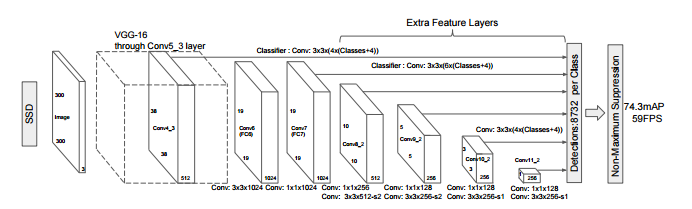
\includegraphics[width=15cm, height=5cm]{images/frameworks/SSD.png}
        \caption[SSD framework]{SSD framework proposed by \citet[p. 24]{Liu2016SSDSS}. The model with the stroked line is the feature extractor network based on VGG19 model and the feature layers are represented in solid lines.}
        \label{fig:Fr-RCNN}
    \end{figure*}
    
    As the CNN reduces the spatial dimension gradually, the resolution of the feature maps also decreases. SSD uses lower resolution layers to detect larger-scale objects and vice-versa. Each convolution predictor in the SSD model produces a fixed set of predictions using the convolution filters \label{feature_maps}. For a feature layer of shape $(m \times n)$ with c channels, the basic kernel for extracting the presence of a potential detection is a $(3 \times 3 \times c)$ shaped kernel. The features extracted can be used to extract either a category or a detection offset ($\Delta C_{x}$, $\Delta C_{y}$, $\Delta w$, $\Delta h$) at every feature map location. In SSD authors used default boxes, which are analogous to anchor boxes in Faster RCNN \cite{Girshick2015} and YOLO \cite{Ren2019}. These default prior boxes encode a considerable amount of prior knowledge about the dataset in their respective shapes. The default boxes are designed to be placed at predefined locations and tiles the generated feature map in a convolutional format so that the position of each box relative to its corresponding cell is fixed. At every cell in the feature map, an offset relative to the default box shape and a class-specific score representing the presence of a class instance are predicted. At a given locations out of k boxes, a total of $(classes+4) \times k$ filters are applied resulting in $\textit{(classes+4)*k*m*n}$ outputs for a $(m \times n)$ feature map. Different aspect ratios and scales for the default boxes result in the effective discretization of the possible bounding boxes.
    
    \begin{figure}[H]
        \centering
        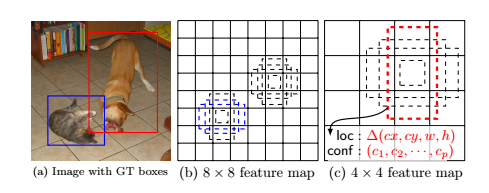
\includegraphics[width=15cm, height=5cm]{images/frameworks/SSD_default_boxes.png}
        \caption[Prior boxes design in \acrshort{ssd}]{Prior boxes defined in different feature layers in SSD framework proposed by \citet[p.24]{Liu2016SSDSS}}
        \label{fig:Fr-RCNN}
    \end{figure}
     
     \subsubsection{Matching Strategy}
     \label{matching_strategy}
     Training an SSD object detection model needs an assignment of ground truth bounding boxes to a fixed size of regressed output boxes. Loss value is calculated using the assigned output boxes and ground truth information and a classical backpropagation are applied in an end-to-end fashion. SSD performance also is dependent on various other tasks like choosing a set of default box aspect ratios and the scales for detection, hard negative mining, and various data augmentation techniques.
     
     We need to assign ground truth boxes to corresponding default boxes. The correspondence is found using Matching Strategy. The default boxes which vary in location, aspect ratio, and scale are matched to ground truths with Jaccard overlap higher than a pre-set threshold. This poses the learning problem to determine multiple bounding boxes with high confidence instead of directly regressing the best fit box with maximum overlap.
     
     \subsubsection{Default box selection}
     \label{default_box}
     The aspect ratios and scales of the prior box in a feature map are to be selected and assigned manually. This selection is dataset-dependent and also defined the number of default boxes in each image. The selection of prior boxes directly affects the performance of the SSD model since they directly affect the matching with the ground truth. The more the positive sample matching is high is the robustness and performance of the SSD object detection model.
     
     \subsubsection{Scales}
     The prior boxes at multiple scales targets objects of different sizes. In the vanilla SSD object detection model the minimum and maximum scales $(s_{\min}, s_{\max})$ are set to 0.2 and 0.9. The scale $S_{k}$ of the $k_{th}$ default box from $m$ feature maps is computed using Equation \ref{scale_setting}.
     
     \begin{equation}
        \label{scale_setting}
        S_{k}=S_{\min }+\frac{S_{\max }-S_{\min }}{m-1}(k-1), k \in[1, m]
     \end{equation}
     
     In the case of SSD300, the largest feature map is from $conv{4_3}$ layer and is assigned a scale of 0.2 and $conv9-2$ has the smallest feature map with a scale value of 0.9 and the rest of the layers has scales assigned evenly. Scale range can be tuned according to the scales of objects of interest present in the dataset.
     
     \subsubsection{Aspect ratios}
     Aspect ratio encodes a knowledge of different object shapes in the dataset. In the original work the aspect ratios are assigned as $a_{r} \in\left\{1,2,3, \frac{1}{2}, \frac{1}{3}\right\}$ for all the multi-scale feature maps. Using the scale and aspect ratio values the width and height of the default box are calculated as $s_{k} \sqrt{a_{r}}, s_{k} / \sqrt{a_{r}}$ accordingly. 
     
     For an aspect ratio of 1 authors also added another scale $\sqrt{S_{k} S_{k+1}}$ to the bounding box. This resulted in a maximum of 6 default boxes at each cell. But, for optimizing the model and improving the inference speeds the first and final two feature maps are assigned with 4 bounding box ratios of 1,2, $\frac{1}{2}$. The aspect ratios and scales of the default boxes of the SSD300 model are shown in Table \ref{tab:priorbox_count}.
     
     \begin{figure}
        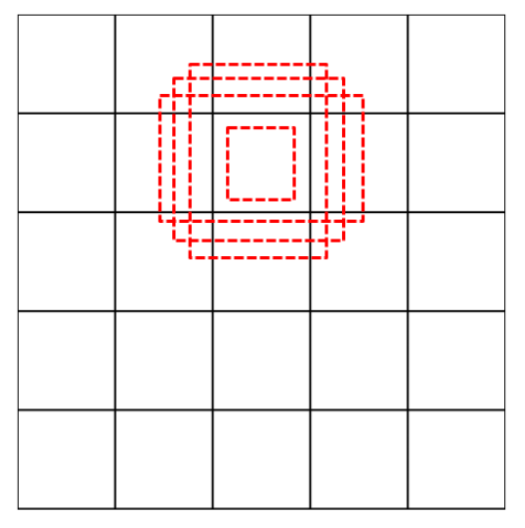
\includegraphics[width=0.46\linewidth]{images/frameworks/feature_maps_5x5.png}\hfill
        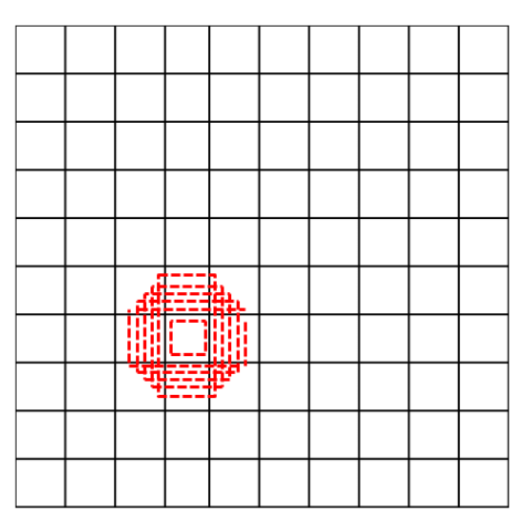
\includegraphics[width=0.475\linewidth]{images/frameworks/feature_maps_10x10.png}
        \caption[Default box design]{Example of default boxes placed for feature maps of size 5x5 and for feature maps of size 10x10}
        \label{fig:bdd100k_samples}
    \end{figure}
     
     \begin{table}[H]
         \centering
         \caption{Table showing the number of default boxes for each multiple feature map layer. Also, observe that the first and last layers have reduced number of default boxes to increase inference speeds}
         \label{tab:priorbox_count}
         \begin{tabular}{|c|c|c|c|c|c|c|c|}
            \hline no of box positions & $38 \times 38$ & $19 \times 19$ & $10 \times 10$ & $5 \times 5$ & $3 \times 3$ & $1 \times 1$ & total boxes \\
            \hline SSD300 & 4 & 6 & 6 & 6 & 4 & 4 & 8732 \\
            \hline
        \end{tabular}
     \end{table}
     
     The optimal scales and aspect ratios are different for different datasets and should be re-designed for usage on a different dataset. As the dataset under consideration is BDD100k \cite{bdd100k} and consists of a very different class distribution in comparison to the VOC dataset. Hence the default boxes are to be tuned for better detection performance.
     
     \subsection{Loss Function}
     Deep learning-based object detection models solve classification and box regression tasks. Training a neural network involves reducing a loss value, which is the difference between the output of the model to the respective ground truth. In the case of SSD, this loss value is quantified using Equation \ref{ssd_loss}. 
     
     For a sample input image $x$, $x^{p}_{ij} = (1,0)$ indicates a score for matching an $i^{th}$ default box with $j^{th}$ ground truth box belonging to a category $p$, $l$ indicates a predicted box and $g$ indicates a ground truth box    
     
    \begin{equation}
        L(x, c, l, g)=\frac{1}{N}\left(L_{\text {conf }}(x, c)+\alpha L_{\text {loc }}(x, l, g)\right)
        \label{ssd_loss}
    \end{equation}
     
    Hence, for object classification a confidence loss ($L_{conf}$) is considered. 
     
    \begin{equation}
        L_{c o n f}(x, c)=-\sum_{i \in \text { Pos }}^{N} x_{i j}^{p} \log \left(\hat{c}_{i}^{p}\right)-\sum_{i \in \text { Neg }} \log \left(\hat{c}_{i}^{0}\right) \quad \text { where } \quad \hat{c}_{i}^{p}=\frac{\exp \left(c_{i}^{p}\right)}{\sum_{p} \exp \left(c_{i}^{p}\right)}
    \end{equation}
     
    While for box regression a Smooth L1 distance between the regressed box and the respective ground truth boxes is used. 
     
    \begin{equation}
        \setlength{\jot}{10pt}
        \begin{gathered}
            L_{l o c}(x, l, g)=\sum_{i \in P o s}^{N} \sum_{m \in\{c x, c y, w, h\}} x_{i j}^{k} \operatorname{smooth}_{\mathrm{L} 1}\left(l_{i}^{m}-\hat{g}_{j}^{m}\right) \\
            \hat{g}_{j}^{c x}=\left(g_{j}^{c x}-d_{i}^{c x}\right) / d_{i}^{w} \\
            \hat{g}_{j}^{c y}=\left(g_{j}^{c y}-d_{i}^{c y}\right) / d_{i}^{h} \\
            \hat{g}_{j}^{w}=\log \left(\frac{g_{j}^{w}}{d_{i}^{w}}\right) \quad \hat{g}_{j}^{h}=\log \left(\frac{g_{j}^{h}}{d_{i}^{h}}\right) \\
            \operatorname{smooth}_{L_{1}}(x)= \begin{cases}0.5 x^{2} & \text { if }|x|<1 \\ |x|-0.5 & \text { otherwise }\end{cases}
        \end{gathered}
    \end{equation}
    
    \section{Uncertainty Quantification in Deep Neural Networks}
    Uncertainty acts as a representation of the trustworthiness of a machine learning model, especially in the case of safety-critical applications. In the context of computer vision, \citet{Kendall2017} proposed two major types of uncertainties, \textit{Aleatoric uncertainty} that arise due to the inherent noise in the data like occlusions, motion blur in an image. \textit{Epistemic uncertainty} is a result of a lack of knowledge on the data, it is observed when an object instance is under or not represented in the dataset used for training the models \cite{Scheirer2013, Scheirer2014ProbabilityMF}. \textit{Aleatoric uncertainty} is an irreducible form of uncertainty, as the main reason for it is noise in collecting or querying the data \cite{Kendall2017}. But, the work proposed by \citet{Lopes2019ImprovingRW} proved that reduction in aleatoric uncertainty is made possible with noise-augmented data but not with lost information in the image. \textit{Epistemic uncertainty} can be reduced by introducing data that might represent the testing conditions.
    
    \subsection{Bayesian Neural Networks}
    \label{BNN_Intro}
    \acrlong{dnn} since their inception are modelled with weights assumed to be point estimates \cite{Scheirer2014ProbabilityMF, Kendall2017, Blundell2015}. This assumption makes the network more deterministic for provided inputs. To address these issues \acrshort{bnn} models the weights as a distribution over the provided dataset $P(w \mid D)$.As a consequence of probability distribution modelling $w$ is considered as a random variable. This inherent randomness in \acrshort{nn} parameters enables the extraction of uncertainty from the \acrshort{nn} model.
    
    Given a dataset $D=\left\{\left(x^{(1)}, y^{(1)}\right),\left(x^{(2)}, y^{(2)}\right), \ldots,\left(x^{(N)}, y^{(N)}\right)\right\}$. The posterior distribution $p(w \mid D)$ can be obtained by applying Bayes theorem.
    
    \begin{equation}
        \label{Bayes_Rule}
        p(w \mid D)=\frac{p(D \mid w) p(w)}{p(D)} \\
    \end{equation}
    
    The datasets available are very large resulting in the calculation of $p(D)$ being intractable \cite{gal2016uncertainty, shridhar2019comprehensive}. Hence, instead of exact modeling of $p(w \mid D)$ researchers proposed to approximate the eight distribution. The approximation can be done using various sampling algorithms like Metropolis-Hastings by \citet{Robert2015} and Markov-Chain-Monte-Marlo (MCMC) by \citet{mcmc}. Though these methods can provide an unbiased approximation, they are slow to converge. Researchers proposed another method called Variational Inference (VI) introduced by \citet{Graves2011} which though provides a slightly biased approximation but converges faster.
    
    \begin{figure}[H]
        \centering
        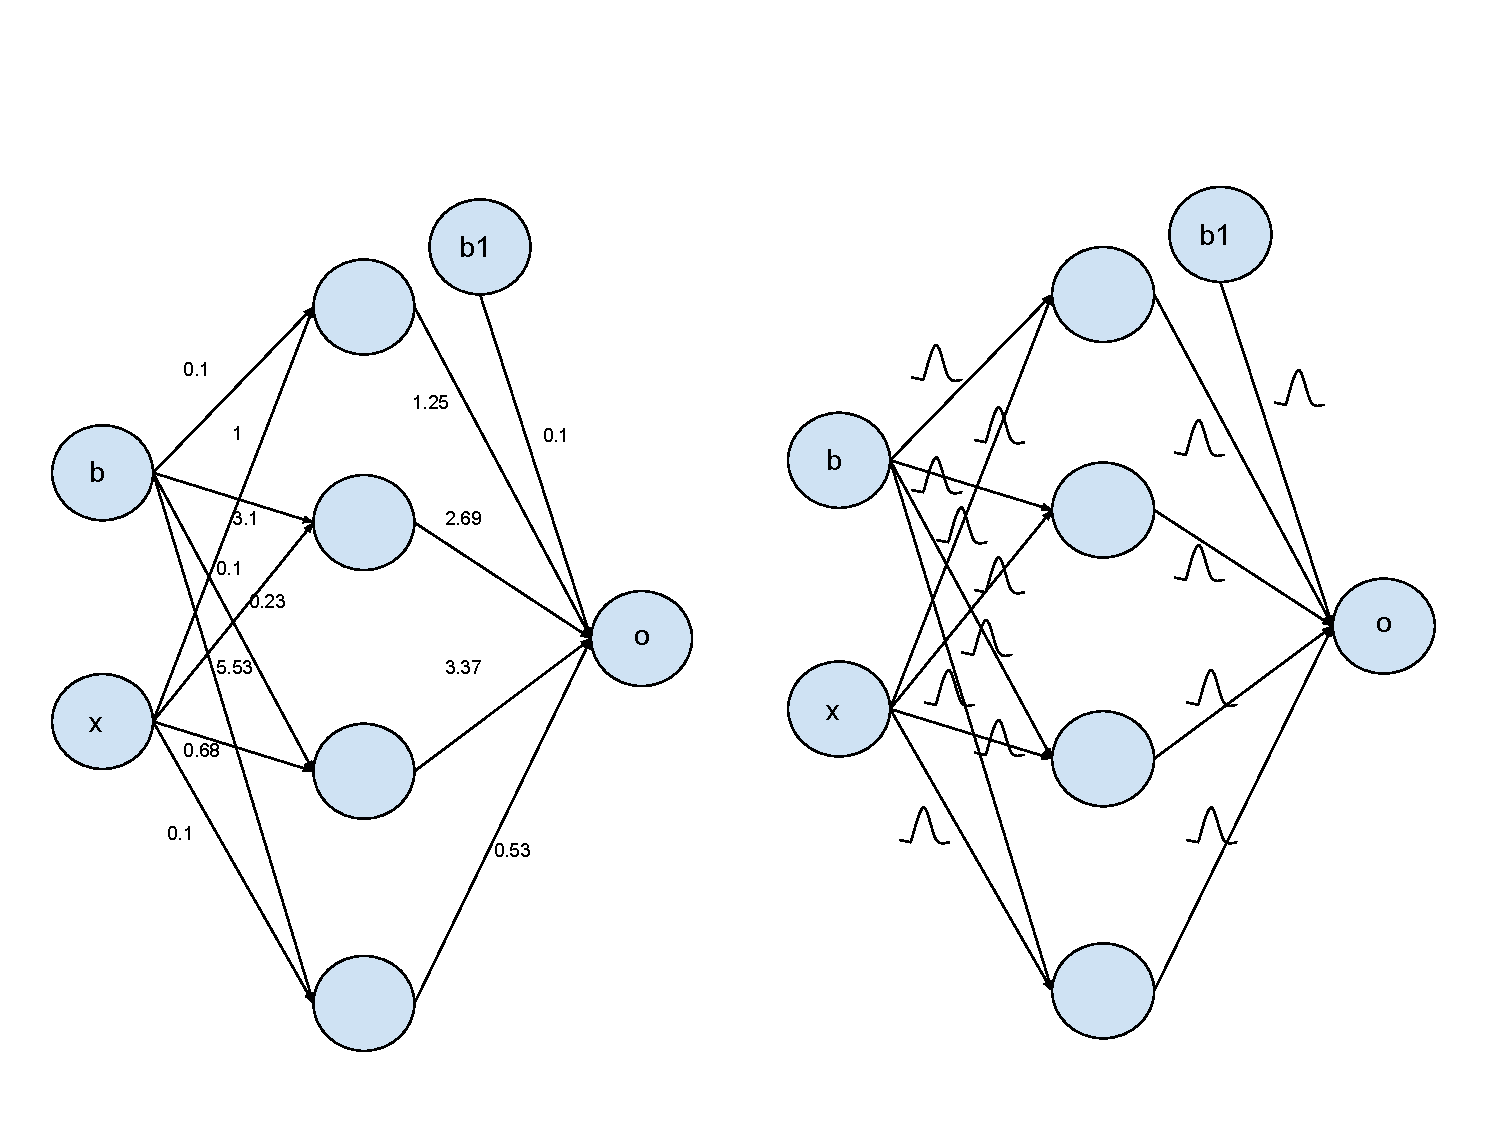
\includegraphics[scale=0.5]{images/frameworks/BNN.pdf}
        \caption[Comparison of Bayesian Neural Network and Fixed-weight Neural Network]{Representation of \acrshort{bnn} with the weights modelled as a gaussian distribution that is parameterized by mean ($\mu$) and variance ($\sigma$) adapted from \citet[pg 3]{shridhar2019comprehensive}}
        \label{fig:BNN}
    \end{figure}
    
    Using VI, $p(w \mid D)$ can be approximated to $q(w)$ parameterized with a mean ($\mu$) and variance ($\sigma$). Using Bayes-by-Backprop proposed by \citet{WBAW1991, Blundell2015} optimize those distributions over the weight parameters to obtain the best approximation. The approximation is judged using Kullback-Leibler (KL) divergence introduced by \citet{Kullback1959} as shown in Equation \ref{KL-D}.
        \begin{equation}
            \label{KL-D}
            \mathrm{KL}(q(x) \| p(x)) \equiv \mathbb{E}_{q(x)}\left[\log \frac{q(x)}{p(x)}\right]=\int q(x) \log \frac{q(x)}{p(x)} d x
        \end{equation}
        
    The posterior calculation problem is now posed as an optimization problem of minimizing the KL-divergence between q(w) and $p(w \mid D)$.
        \begin{equation}
        \setlength{\jot}{10pt}
        \label{log_calc}
            \begin{aligned}
            \mathrm{KL}(q(w) \| p(w \mid D)) &=\mathbb{E}_{q(w)}\left[\log \frac{q(w)}{p(w \mid D)}\right] \\
            &=\int q(w) \log \frac{q(w)}{p(w \mid D)} d w \\
            &=\int q(w) \log \frac{q(w) p(D)}{p(D \mid w) p(w)} d w \\
            &=\int q(w) \log \frac{q(w)}{p(w)} d w+\int q(w) \log p(D) d w- \int q(w) \log p(D \mid w) d w \\
            &=\operatorname{KL}(q(w) \| p(w))+\log p(D)-\mathbb{E}_{q(w)}[\log p(D \mid w)]
            \end{aligned}
        \end{equation}
        
    The optimal parameters $\theta^{opt}$ parameterized with a respective mean and variance ($\mu , \sigma$) are defined as  
        
        \begin{equation}
        \setlength{\jot}{10pt}
        \label{optim_param}
            \begin{aligned}
            \theta^{opt} &=\operatorname{argmin}_{\theta} K L[q(\mathbf{w} \mid \theta) \| P(\mathbf{w} \mid \mathfrak{D})] \\
            &=\operatorname{argmin}_{\theta} \int q(\mathbf{w} \mid \theta) \log \frac{q(\mathbf{w} \mid \theta)}{P(\mathbf{w} P(\mathfrak{D} \mid \mathbf{w}))} \\
            &=\operatorname{argmin}_{\theta} \mathbf{K L}[q(\mathbf{w} \mid \theta) \| P(\mathbf{w})]-\mathbb{E}_{q(\mathbf{w} \mid \theta)}[\log P(\mathfrak{D} \mid \mathbf{w})]
            \end{aligned}
        \end{equation}
        
    With the availability of $q(w)$, an approximation of $p(w \mid D)$ obtained. We can infer an output $y^{*}$ for any given input $x^{*}$ by integrating over the weights available as shown in Equation \ref{Bayesian inference}.
    
        \begin{equation}
            \label{Bayesian inference}
            p\left(y^{*} \mid x^{*}, D\right) \approx \int p\left(y^{*} \mid x^{*}, w\right) q(w) dw 
            & \approx \frac{1}{K} \sum_{k=1}^{K} p\left(y^{*} \mid x^{*}, w^{k}\right)
        \end{equation}
    
    \subsection{Deep Ensembles}
    Deep Ensembles proposed by \citet{Lakshminarayanan2017} are an ensemble of multiple deep learning models. All the ensembled models are with the same model architecture, each of these models is initialized randomly and trained using a dataset that is randomly shuffled. In general, an ensemble performs model combination in contrast to Bayesian Model Averaging. Hence, ensembles do not assume that a perfect model is present in the trained models. \citet{Lakshminarayanan2017} also investigated the usage of these proposed deep ensembles to estimate inherent uncertainty in the models.
    
    For an ensemble of size \textit{\textit{N}} and a model \textit{\textit{M}}, the schema used by \citet{Lakshminarayanan2017} is:
    
    \begin{enumerate}
        \item Each member of \textbf{\textit{N}} is initialized with weights and biases independently
        \item Train each member in the ensemble with randomly shuffled dataset
        \item Final output from the ensemble is produced by the averaging model
    \end{enumerate}

    \subsubsection{Deep Sub-Ensembles}
    \label{deepsubensembles}
    Deep Sub-Ensemble proposed by \citet{ValdenegroToro2019} divides a neural network model into two sub-networks, the trunk network \textbf{\textit{T}} and a task network \textbf{\textit{K}}. Hence, for an input $x$ a neural network can be represented as \textbf{\textit{K(T(x))}}.
    
    From the above representation, an Ensemble can be represented as $K_{i}(T_{i}(x))$, where i $\in$ (1,...,N). From the work done by \citet{ValdenegroToro2019}, the author followed the work on Bootstrapped DQN \cite{Osband} fixed the trunk network weights $(T_f)$ and trained various instances of the task models $K_{i}(x)$, where i $\in$ (1,..., N). In a nutshell, Deep Sub-Ensemble contains a fixed trunk network $T_f$ and multiple instances of task network $K_{i}$ which makes the ensembling process computationally less expensive and a real-time inference of both high-quality detection and uncertainty values is possible with GPU parallel computation ability. 
    
    \begin{figure}[H]
         \centering
         \begin{subfigure}[b]{0.495\textwidth}
             \centering
             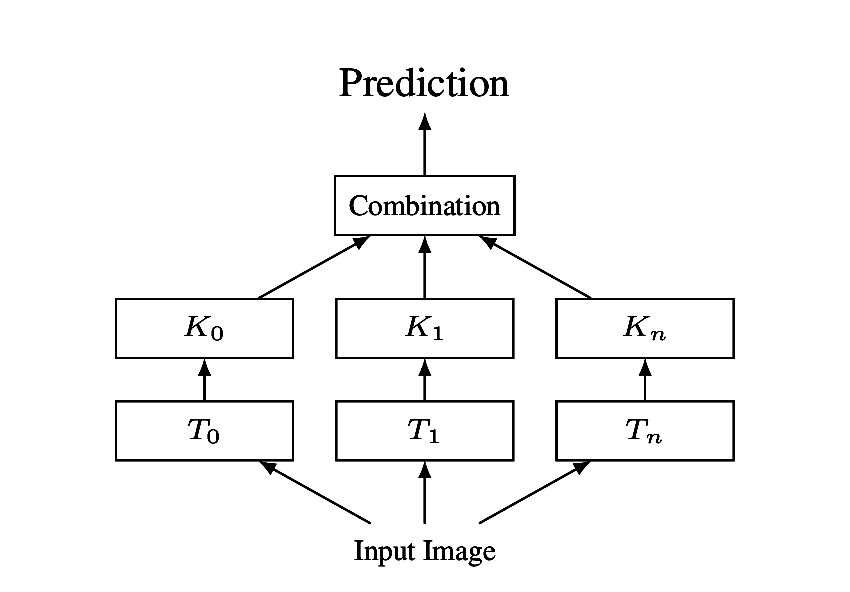
\includegraphics[width=\textwidth]{images/frameworks/ensembles.png}
             \caption{Ensemble}
             \label{fig:Ensemble}
         \end{subfigure}
         \hfill
         \begin{subfigure}[b]{0.495\textwidth}
             \centering
             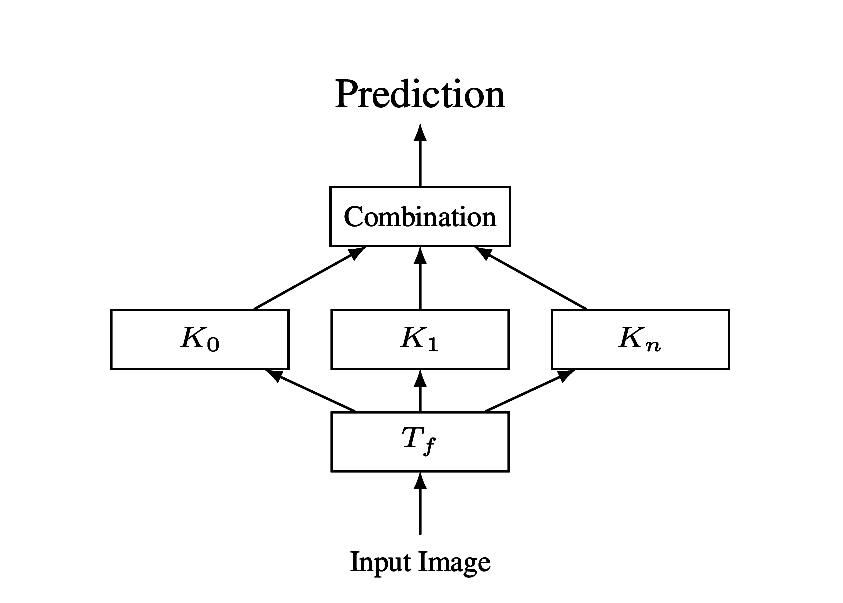
\includegraphics[width=\textwidth]{images/frameworks/subensembles.png}
             \caption{Sub-Ensemble}
             \label{fig:Sub-Ensemble}
         \end{subfigure}
            \caption[Ensemble vs Sub-Ensemble]{Comparision of Ensembles and Sub-Ensembles, observe that there is only one trunk network in Sub-Ensembles which leads to a decrease in need for computational resources needed \cite[p.2]{ValdenegroToro2019}}
    \end{figure}
    
\end{document}
